\author{Andrei Tkachuk}

\part{Обыкновенные дифференциальные уравнения и их системы}
\section{Введение. Дифференциальные уравнения 1-го порядка}

\begin{Def}[Дифференциальное уравнение]
    Уравнение вида $F(x, y, y', y'', \dots, y^{(n)}) = 0$ называют обыкновенным дифференциальным уранением n-го порядка. Решением называют функцию $y = y(x)$, которая n раз дифференцируема на интервале I: 
    \[
        F(x, y(x), y'(x), \dots, y^{(n)}(x)) = 0
    \]
\end{Def}

\begin{Def}[ДУ разрешённое относительно старшей производной]
    Если дифференциальное уравнение имеет вид
    \[
        y^{(n)} = f(x, y, y', \dots, y^{(n - 1)})
    \]
    то тогда его называют обыкновенным дифференциальным уравнением n-го порядка разрешённого относительно старшей производной 
\end{Def}

\begin{Example}[моделный]
    Пусть $f(x) \in C'_{(a, b)}, \, y' = f(x)$ --- дифференциальное уравнение n-го порядка, разрешённое относительно 1й производной.
    \begin{floatingfigure}[l]{50mm}
        \noindent
        \hfil
        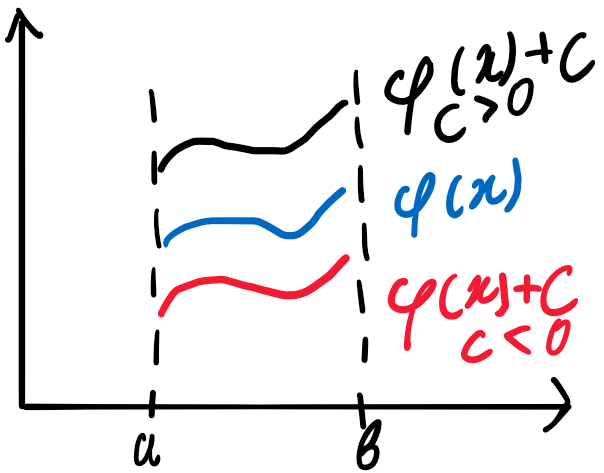
\includegraphics[width=45mm]{pictures/2_1_1.png}
        \hfil
    \end{floatingfigure}
    Если $y = y(x)$ решение, то
    \begin{gather*}
        y'(x) = f(x)\\ 
        y = \int{f(x)dx} + C = \varphi(x) + C \quad x \in (a, b)
    \end{gather*}
    Если $y = \psi(x)$ решение ДУ, то 
    \[
        \exists C,\; \forall x \in (a, b) \quad \psi = \varphi(x) + C
    \]
    Для любого $(x_0,\, y_0)$ в полосе, т.е. для $x_0 \in (a, b)$ существует решение $y = \varphi(x) - \varphi(x_0) + y_0, \, (y_0 \in \bb{R})$
\end{Example}

    Таким образом мы видим, что для одного дифференциального уравнения существует множетсво решений. Для конкретизации задачи используют условие Коши.

\begin{Def}[Задача Коши]
    Система вида
    \[
        \begin{cases}
            y' = f(x, y)\\
            y|_{x = x_0} = y_0 \quad (\text{конкретизация первообразной})
        \end{cases}
    \]
    Называется условием Коши, а задача о поиске решения это задача Коши
\end{Def}

    \begin{figure}[h!]
        \noindent\centering{
            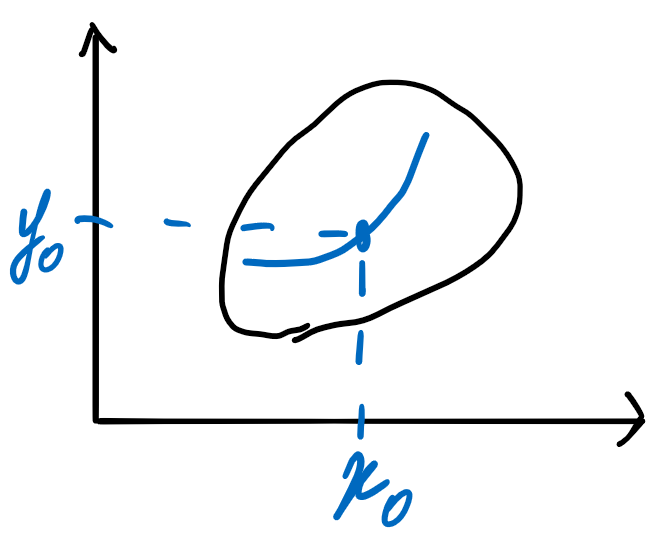
\includegraphics[width=55mm]{pictures/2_1_2.png}
            \caption{}
        }
    \end{figure}

\begin{Th}[Сущ. и ед. решения задачи Коши для ДУ 1го порядка]
    Пусть $f(x, y) \in C(U(M_0))$ и $\exists f'_y(M) \in C(U(M_0))$. Тогда существует такая $\delta > 0$ и существует решение $y' = y(x) \in U_\delta(M_0)$ задачи Коши c соответвующим условием $y' = f(x) \quad y(x_0) = y_0$ и такое решение в $U_\delta(x_0)$ единственно
\end{Th}
\begin{Proof}
    Принимаем без доказательств
\end{Proof}

\begin{Def}[Поле направлений ДУ]
    Пусть 
    \[
        y' = f(x, y), \quad f(x, y) \in C(D)
    \]
    $M_0(x_0, y_0)$ --- любая внутренняя точка области $D$. Запишем уравнение касательной к графику решения задачи Коши
    \[
        l_0 : Y-y_0 = f(x_0, y_0)\,(X-x_0)
    \]
    а задача Коши
    \[
        \begin{cases}
            y' = f(x, y)\\
            y|_{x = x_0} = y_0
        \end{cases}
    \]
    Пусть $\vec{\tau}$ --- единичный вектор касательной. Тогда множество $\{\vec{\tau}\}$ --- поле направлений
\end{Def}

\begin{figure}[h!]
    \noindent\centering{
        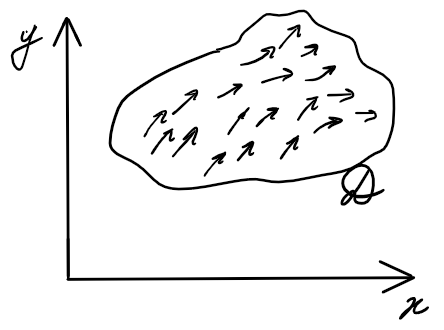
\includegraphics[width=55mm]{pictures/2_1_3.png}
        \caption{Поле направлений}
    }
\end{figure}

Вместе с понятием поля направлений вводят (для удобства) такую вещь как изоклины, т.е. линии, вдоль которых поле имеет одно и тоже направление. Задаётся уравнением $f(x, y) = C$\\

Тут важно заметить, что понятие поля направлений очень сильно связано с физикой, так как с помощью них можно легко описывать физические поля (эклектрическое, магнитное).

\textcolor{cyan}{С помощью полей направлений доказывается теорема о единственности задачи Коши.}

\begin{Example}
    Дано: 
    \[
        y' = \frac{y}{x}
    \]
    Требуется построить поле направлений.\\
    Решение.\\
    \begin{floatingfigure}[2]{34mm}
        \noindent
        \hfil
        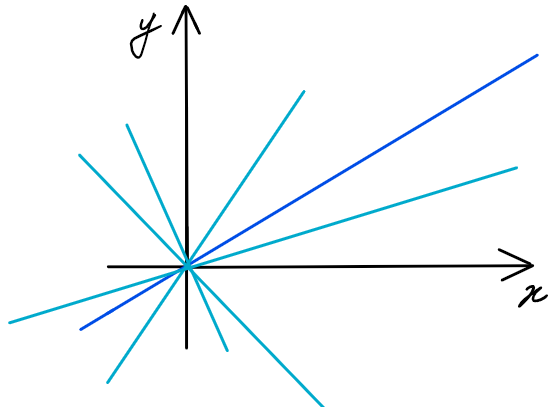
\includegraphics[height=24mm]{pictures/2_1_4.png}
        \hfil
    \end{floatingfigure}
    Изоклины для данного ДУ задаются уравнением 
    \[
        \frac{y}{x} = C
    \]
    
    Получается, изоклины представляют собой прямые, проходящие через начало координат. Уравнение изоклин $y = C\,x$. Если подставлять пары $(x,\; y)$, то мы заметим, что вектора поля направлений совпадают с изоклинами.\\
    Таким образом поле направлений состоит из множества прямых, проходящих через начало отсчёта (Точка (0, 0) выколотая).
\end{Example}

\begin{Example}
    Дано
    \[
        y' = -\frac{x}{y}
    \]
    Требуется построить поле направлений.\\
    Решение.\\
    Изоклины для данного ДУ задаются уравнением 
    \[
        -\frac{x}{y} = C
    \]
    Аналогично примеру выше, видим что изоклины проходят через начало координат.\\
    Рассмотрим несколько изоклин.
    \begin{enumerate}
        \item $C = -1$, тогда $y = x$. Прямая в первой и третьей четверти. Для неё значение углового коэфициента $k = -1$. Следовательно угол равен $\frac{3\,\pi}{4}$ для первой четверти
        
        \item Рассмотрим $C \in (-\infty;\, -1)$, тогда нетрудно заметить, что угол $\varphi$ соответственно изменялся для первой четверти от $\frac{\pi}{2}$ до $\frac{3\,\pi}{4}$ (оба не включительно).
        
        \item Рассмотрим $C \in (-1;\, 0)$. Тогда угол $\varphi$ соответственно изменялся для первой четверти от $\frac{3\,\pi}{4}$ до $\pi$.
    \end{enumerate}
    \begin{figure}[h!]
        \noindent\centering{
            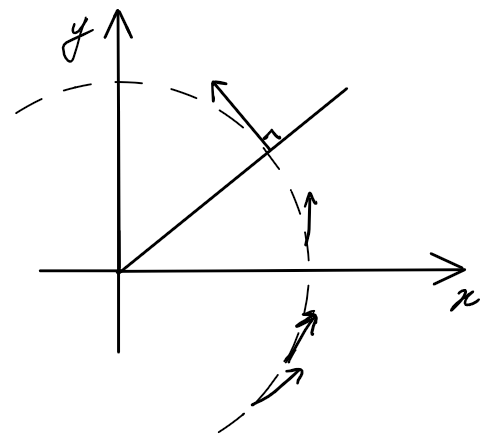
\includegraphics[width=45mm]{pictures/2_1_5.png}
            \caption{Иллюстрация примера}
        }
    \end{figure}
\end{Example}

\begin{Def}[Общее решение]
    Пусть $y' = f(x, y)$ --- ДУ первого порядка. Функция $y = \varphi(x, C)$ называется общим решением этого ДУ если:
    \begin{enumerate}
        \item $\forall C \in \bb{R}$ $y$ как функция от $x$ является решением ДУ
        
        \item Для любого решения $y = y^*(x)$ 
        \[
            \exists C^* \in \bb{R}, \quad y^*(x) \stackrel{(x)}{\equiv} \varphi(x, C^*)
        \]
    \end{enumerate}
\end{Def}

\begin{Note}
    Уравнение $\Phi(x, y, C) = 0$ --- называется общим интегралом ДУ. $y' = f(x, y)$ если:
    \begin{enumerate}
        \item всякая неявная функция $y = y(x, C)$ при фиксированном $C$ является решением ДУ
        \item всякое решение задаётся неявной функцией $y = y(x, C^*)$ для некоторого $C^*$
    \end{enumerate}
\end{Note}

\begin{Example}
    Для $y' = \frac{y}{x}$ очевидно из рисунка, что общее решение
    \[
        y = C \, x
    \]
\end{Example}

\begin{Example}
    Для $y' = -\frac{x}{y}$ очевидно из рисунка, что общий интеграл 
    \[
        x^2 + y^2 = C^2
    \]
    Общее решение отсутствует
\end{Example}

\begin{Note}
    Точка особая, если нарушается существование и единственность задачи Коши
\end{Note}

\begin{Note}
    $y = \varphi(x, C)$ --- <<общее>> решение, $y = \hat{y}(x)$ --- особое решение по отношению к общему решению.
\end{Note}

\begin{Note}
    Дано $y' = f(x)$, тогда 
    \[
        y = \int{f(x)\,dx} + C
    \] 
    называется решением ДУ <<в квадратурах>>.\\
    Важно заметить, что интегралов может быть несколько. Например,
    \[
        y^{(n)} = f(x)
    \] 
    интегрируется в квадратурах, через последовательное интегрирование. Другим примером является сумма интегралов.
\end{Note}